\chapter{Introduction}
\label{chap:intro}

\makeatletter
\newenvironment{chapquote}[2][2em]
{\setlength{\@tempdima}{#1} \def\chapquote@author{#2} \parshape 1
  \@tempdima \dimexpr\textwidth-2\@tempdima\relax \itshape}
{\par\normalfont\hfill--\
\chapquote@author\hspace*{\@tempdima}\par\bigskip}
\makeatother

\begin{chapquote}{Alan Turing}
  ``I propose to consider the question: Can machines think?''
\end{chapquote}
The ultimate goal of image understanding is to transfer visual
signals (images/videos) into abstract symbolic descriptions of the
world which are helpful for decision making.
However, understanding images is a not trivial task for machines.
In order to handle various complicated scenarios, researchers divide
image understanding into different computer vision tasks: pedestrian
detection for autonomous driving, face recognition for security
system, and image retrieval for image searching engines.

For many applications, knowing when, where, and in which direction a
picture was taken is important to understand the world. However, most
images does not carry such information, thus we need to develop
algorithms to dig them up.  We refer to the task of estimating these
properties as {\em geo-calibration}.
Most recent work of geo-calibration focus on deterministic systems, 
which have some drawbacks: 1) they can not model the inherent
uncertainties from images of ambiguous scenes, and 2) they can not be
used by applications that take probabilistic inputs. To address
these problems, we propose to build probabilistic models for camera
geo-calibration.

We also show that learning to geo-calibrate a camera is helpful for
high-level feature extracting. Feature engineering is essential for
image understanding. In recent years, learning based approaches for
high-level feature extracting like deep neural nets have drawn a lot
of attention due to the fact that they do not need any expert
knowledge about the target data. However, most of these feature
learning methods heavily relies on manually labeled data. In our
thesis, we presented alternative ways to learn high-level image
representations when the manually labeled data is either insufficient
or absent.

\section{Background}

\subsection{Geo-Calibration of Outdoor Images}
Automatic image geo-calibration of outdoor images continues to grow in
importance as a direct result of the increasing amount of imagery
available via the Internet.  Solving this problem is of great value
for a wide variety of fields, with potential applications ranging from
the forensic sciences~\cite{stylianou13jane} to environmental
monitoring~\cite{zhang2012mining}.  Conceptually the geo-calibration
task includes: identifying the camera pose ({\em pose estimation}),
the camera geographic location ({\em geo-localization}), and the time
the query image was captured ({\em time estimation}).

\begin{itemize}[noitemsep]

\item \textbf{Pose Estimation:}
Li et al.~\cite{li2012worldwide} exploit geo-registered 3D points
clouds to estimate camera pose.
Vo \etal~\cite{vo2016localizing} propose a geo-localization network
that can regress the geo-orientation angle of the camera.
Agarwal \etal~\cite{agarwal2015metric} keep track of the camera pose
changes by matching SIFT~\cite{lowe1999object} feature points detected
between the input image and Google Street View panoramas.
%
Horizon line detection is an essential step for some pose
estimation algorithms, because horizon lines are closely related to
camera pitch and roll angles.
%If the camera focal length is known, one can compute the camera pitch
%and roll angle from the horizon line.
Collins and Weiss~\cite{unitsphere1990} formulate horizon line
detection as a statistical estimation problem on the Gaussian Sphere,
which is similar to the geometry we use.  More recent work has
explored the use of dual space~\cite{alignment2014,dualspace2013}
representations. Among the clustering-based approaches, Xu et
al.~\cite{kitware2013} improve this pipeline by introducing a new
point-line consistency function that models errors in the line segment
extraction step.
\newline

\item \textbf{Geo-Localization:}
Extracting location-dependent features from
image data has drawn a great detail of attention from the vision
community~\cite{jacobs07geolocate, jacobs11geolocate,
jacobs08geoorient}. The common trend amongst these methods is that
they take advantage of a large dataset of geo-referenced images. Hays
and Efros~\cite{hays2008im2gps} use a data-driven scene matching
approach to localize a query image using a large dataset of geo-tagged
images.  Doersch \etal~\cite{doersch2012what} extract
location-dependent features that capture the relative appearance
differences of large cities.  Lin et al.~\cite{lin2013cross} localize
a ground-level image by learning the relationship between pairs of
ground and aerial images \footnote{In the context of our thesis, we
do not distinguish between the satellite imagery and the aerial
imagery} of the same location. Other techniques focus
on urban environments and infer location using local image
descriptors~\cite{schindler2008detecting,snavely2006photo}.
Many other cues exist, such as the
skyline~\cite{baatz2012large,ramalingam2009geolocalization}, sky
appearance~\cite{lalonde2010sun,workman2014rainbow}, and
shadows~\cite{junejo2008estimating,wu2010geo}.
\newline

\item \textbf{Time Estimation:}
Matzen and Snavely~\cite{matzen2014scene} predict
timestamps for photos by matching against a time-varying
reconstruction of a scene.  Hill~\cite{hill1994elephant} estimate the
time of the day by measuring the light intensity profiles captured by
cameras. Methods are proposed to date the
year book photos by analyzing human
appearance~\cite{salem2016face2year,ginosar2015century}. Lee
\etal~\cite{linking2015iccp} find visual paterns in the buildings,
relate them to certain time periods.
\newline

\end{itemize}

\subsection{Deep Learning in Geo-Calibration}
In recent years, deep neural networks (DNNs) were proven to be
extremely successful in many computer vision areas. 
It is widely accepted that DNNs have excellent performance in
high-level visual feature learning.
This valuable ability provides researchers powerful tools to
solve the challenging geo-calibration tasks.
Weyand and Kostrikov \etal~\cite{planet} propose a convolutional
network to predict the geographic location of the input
image. Walch \etal~\cite{walch2017image} aggregate learned CNN
features with LSTM to generate global image representation for camera
localization.  In pose estimation aera, Work~\cite{zhai2016horizon,
workman2016horizon, hold2017perceptual} has been done to to identify
the horizon line with CNNs (one can derive the camera roll and pitch
angles from the horizon line position giving the camera focal length).

Closely related to camera geo-calibration, studies also have been done
to identify the camera intrinsics using deep neural networks.
Workman \etal~\cite{workman2015deepfocal} develop a CNN to estimate the camera
focal length. Kendall \etal~\cite{kendall2015convolutional} propose a
neural network that can identify 6-DOF camera parameters, but their
method only limited to specific scenes.


\subsection{Ground-to-Aerial Geo-Calibration}
Data-driven scene matching approaches are widely used to for
geo-calibration.
When localizing a camera, data-driven algorithms search for k-nearest
neighbors of the query image in the database of the geo-tagged imagery.
To reduce the work of querying, the searching process is usually
carried out in some feature space with applicable number of  
dimensions~\cite{im2gps, li2010location,zamir2010accurate}.
However, as items found in most reference dataset, geo-tagged
ground-level images collected from the internet are usually noisy and
sparse in geographic space. To achieve more accurate geo-calibration
results, we need alternative image resources with more accurate
geographic tags and denser spatial coverage.

Benefited from the fast growing monitoring satellite and drone markets,
the geo-tagged aerial imagery becomes more publicly accessible
than ever before. Aerial imagery downloading services like
Microsoft Bing Map provide aerial images of various
resolutions, which can cover most areas of the world with accurate
geographic tags, making aerial imagery a rich source for
reference database. We refer to the geo-calibration methods
which use the aerial imagery as geographic reference as
ground-to-aerial geo-calibration.

Recent work on ground-to-aerial
geo-calibration~\cite{lin2013cross,lin2015learning,workman2015geocnn,workman2015wide}
has shown that convolutional neural networks are capable of extracting
features from geo-tagged aerial imagery that can be matched to
features extracted from the ground imagery.  Vo
\etal~\cite{vo2016localizing} extend this line of work, demonstrating
improved geo-localization performance by applying an auxiliary loss
function to regress the ground-level camera orientation with respect
to the aerial image. Hu and Feng \etal~\cite{mh2018cvm} achieve the
state-of-the-art performance in geo-localization by extracting
cross-domain global features using the
NetVLAD~\cite{arandjelovic2016netvlad} technique.


\subsection{Geo-Calibration for Feature Learning}

Automatic feature engineering has drawn a lot of attention over the
past years. Compared to the manual feature engineering,
automatic feature engineering approaches are able to to learn useful
features without strong expert knowledge about the data. Among these
approaches, deep neural networks are wildly accepted by researchers as
good tools to learn high-level image representations.  The most
commonly used approach for deep feature learning is full supervision,
which usually requires manually annotated
data~\cite{yosinski2014transferable,zhou2016learning,wen2016discriminative}.
Unfortunately, such data is not always available for certain tasks.
In contrast, unlabeled data is offen plentiful (\ie cellphone photos
in Instagram or Youtube videos).

To exploit these unlabeled data, recent work has explored
self-supervision methods (sometimes referred to as unsupervised learning or
pretext tasks) for training deep neural networks that capture useful
visual representations~\cite{doersch2015unsupervised,pathak2016context}. 
These methods typically
exploit some known quantity of the data (e.g., pixel color values) to
avoid expensive manual annotation. As a byproduct, a useful visual
representation is learned.
For example, Zhang et al.~\cite{zhang2016colorful} show how image
colorization (synthesizing colors for a grayscale image) is a powerful
pretext task for learning visual representations. Pathak et
al.~\cite{pathak2017learning} exploit low-level motion-based grouping
cues for unsupervised feature learning.  
%
As new learning technique address the lack of massive amounts of
labeled data, domain adaptation adapt the feature generating model to
another feature domain so that it improve the performance when dealing
with new input
data~\cite{fernando2013unsupervised,fernando2015joint,saenko2010adapting,wang2016actions,tinghui2016flow}.
Duan \etal~\cite{duan2012learning} proposed to learn a linear
projection to transfer from the source feature subspace to the target
subspace. Sohn \etal~\cite{sohn2017unsupervised} improved the
performance of video face recognition using an adversarial-based
approach to adapt the network to unlabled video imagery.

\section{Main Contributions}

\begin{figure}
  \centering
  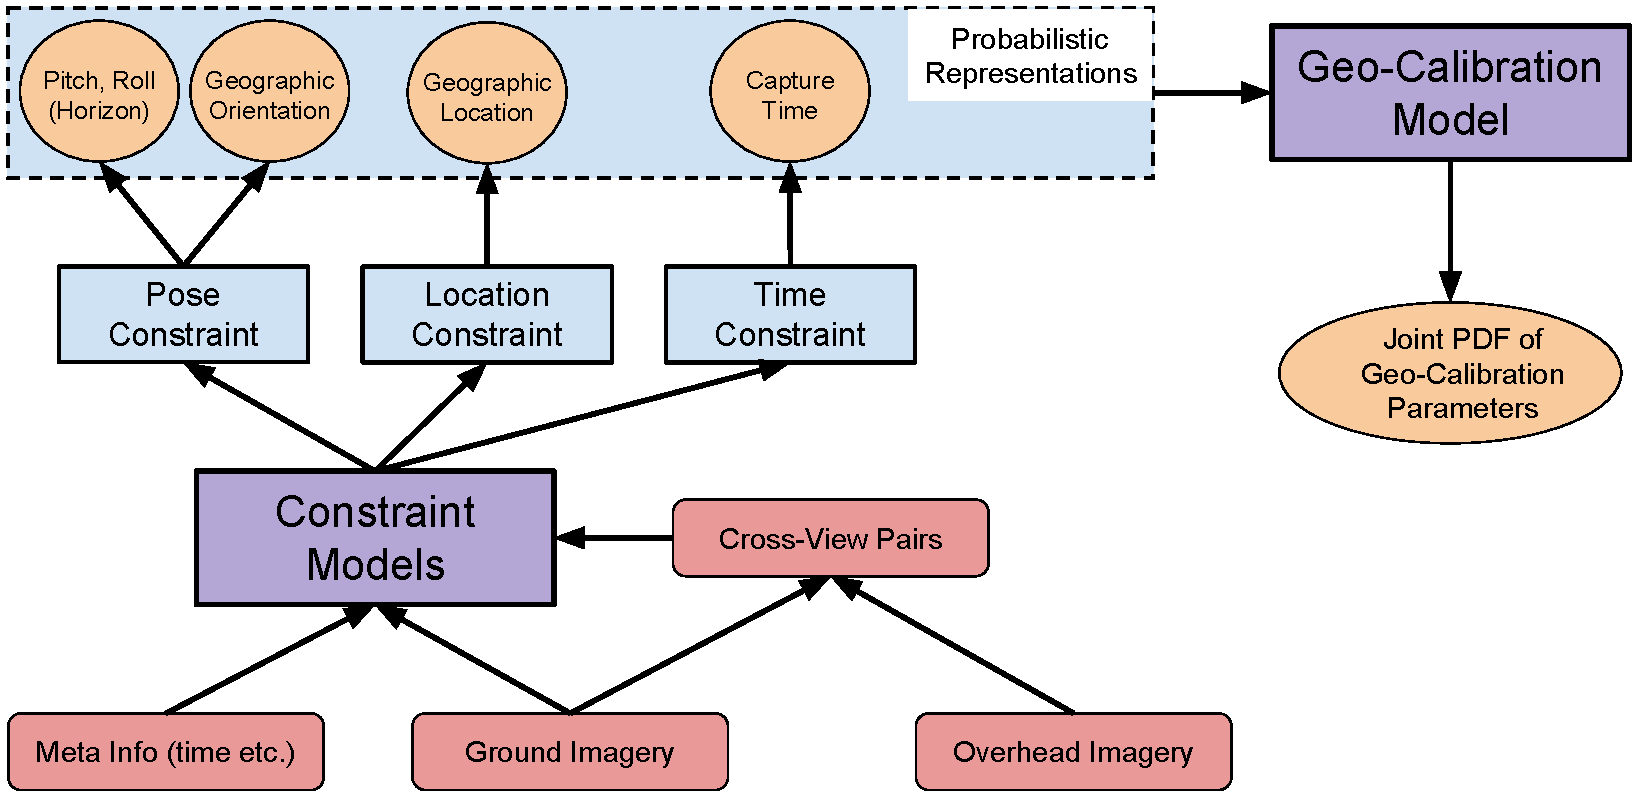
\includegraphics[width=\linewidth]{introduction/architecture}
  \caption{A simplified flowchart of our approach. The algorithm
inputs (images, time and manual annotations) are fed to different
constraint models which work as constraint functions. 
The probabilistic distribution over complete geo-calibration
parameters are then simulated jointly by fusing these constraint
functions in a general model for geo-calibration.}
  \label{fig:intro:architecture}
\end{figure}

We make contributions in three main areas: 1) We proposed a general
probabilistic model to jointly estimate the geo-calibration
parameters, 2) we decompose the full geo-calibration into several
partial geo-calibration tasks, each of which provides a strong
constraint function that fits in the general model, and 3) we show
that learning to geo-calibrate a camera is helpful for high-level
image feature extraction.

The first two contributions consist of our main approach. Our
algorithm feeds inputs (images, time and manual annotations) to
different constraint models, which work as constraint functions. Then
we fuse these constraint functions to simulate the joint distribution
over the complete geo-calibration parameters. The flowchart of
our approaches refers to \figref{intro:architecture}.

Furthermore, we also explore to learning high-level
visual features and geo-calibrating cameras simultaneously.
We believe that the geo-calibration parameters are closely related to
the image representation. 
Imagine the process of a human doing geo-localization, one could
roughly guess where a photo was taken when she sees an polar bear on
an iceberg on it. In this process, learning high-level features
becomes a necessary step of abstracting visual hints to localize
the camera.
Based on this belief, we designed network to learn useful visual
features by exploiting geographic information, which provides new ways
for automatic feature learning.


\subsection{General Probabilistic Model for Geo-Calibration}
The complete camera geo-calibration detects the camera
geographic location, pose, and focal length of the camera.  We
design a general model to estimate the probability over these
geo-calibration parameters: First, we model the relationship between the
image projection of the scene and the geo-calibration parameters. This
relationship can be described by the pin-hole model, and
the geographic location of the camera.
We then construct a scoring function to measure the ``fitness'' between the
calibration parameters and the observation of the image. 
The scoring function is proportional to the probability distribution
of the camera parameters. We propose a Markov Chain Monte
Carlo (MCMC) sampling approach to approximate the underlying
probability distribution over the full geo-calibration of the camera.
Our model is a general architecture, which can take different
constraints to form the scoring function. The details about this model
can be found in \chapref{mcmc}.

\subsection{Developing Constraint Functions}
In our general model, the scoring function is defined as a linear
combination of multiple constraint functions.
In the rest of the work, we focus on developing good constraint
functions for different set of calibration parameters. 

\begin{itemize}[noitemsep]
  \item \textbf{Constraint for Horizon Line and Vanishing Points:}
  We first estimate camera roll and pitch angles. Assuming the intrinsic
  parameters are known, camera roll and pitch angles can be
  derived from the horizon line position in the image. Compared to
  directly detecting the camera pose, identifying horizon line is easier
  because it is tightly related to the appearance
  of the scene. In our work, we create a new method using CNN to
  estimate the prior distribution of the horizon line. We assign
  a probability to each horizon line by measuring their consistences
  with vanishing points detected using traditional statistic methods.
  We present the algorithm details in \chapref{fasthorizon}.
  \newline

  \item \textbf{Constraint for Time and Coarse Geographic Locations:}
  In this work, we demonstrate to estimate the capture time and the
  camera geographic location given the input image.
  Our network has two heads to predict the image
  capture time and the geographic location jointly.
  For time estimation, our network is able to predict the
  joint distribution over the month of the year and the global hour of the
  day when the input image has been captured.
  For camera geo-localization, We provide two approaches to obtain the
  probability distribution over the camera geographic location. Most
  straightforwardly, our network estimate the categorical distribution
  over location of the world, which is represented as a $N \times M$
  meshgrid. Better results can be procured with image capture time as
  auxiliary input (if it is known). 
  %Our algorithm can also compute the probability at arbitrary
  %geographic location, with lower accuracy than the straightforward
  %method.
  We will present the algorithm details in \chapref{whenwhere}.
  \newline

  \item \textbf{Constraint for Fine Geographic Locations and Orientations:}
  In our previous method, we present that our algorithm can estimate
  the camera location distribution in low-res world division. In this
  work we focus on refining the geo-localization results with the help
  of overhead imagery and on estimating geo-orientation of the camera. 
  We first learn to segment the ground scene from its paired aerial image.
  When refining the camera geographic location, we compare the
  semantic layout of the ground image with the semantic layout
  transferred from overhead images, which are sampled in different
  locations and orientation angles. The optimal prediction is found when the
  semantic layouts from these two sources match best. For probabilistic
  outputs, we assign a score to each location and orientation setting,
  based on how well the semantic layouts match to each other. We will
  present the algorithm details in \chapref{crosstransf}.
  \newline

\end{itemize}


\subsection{Geo-Calibration for Feature Learning}
Our methods also focus on lavaging the camera geographic information to
deal with the challenges of lacking manually annotated data during DNN
training. The insight is that the camera geographic information
encodes semantic information because it is related to the
appearances of the scenes.

\begin{itemize}[noitemsep]
  \item \textbf{Ground-to-Aerial Feature Learning:}
  Current machine learning methods address problems that involves mostly
  the ground-level imagery. Tons of dataset targeting on ground imagery are
  annotated while much fewer are done for the satellite/aerial imagery. In
  \chapref{crosstransf}, we proposed a method to learn the aerial image
  semantic segmentation with only ground-level ground truth. Our method
  exploits the spatial correspondences between images in cross-view
  pairs. 
  In this work, we try to transfer the semantics from the ground
  imagery to the aerial imagery by identifying the latent geometry
  correspondences between these two. Similar to the monocular depth
  estimation methods that driven by the technique called {\em
  Reprojection Losses}~\cite{garg2016unsupervised,
  godard2017unsupervised,zhou2017unsupervised, yan2016perspective}, our
  network learns to geometrically project pixels from the aerial
  images to the ground images, and to segment the aerial images
  jointly.
  \newline

  \item \textbf{Geo-Temporal Feature Learning:}
  In \chapref{whenwhere}, we demonstrate that our algorithm is able to
  learn geo-temporal image representations with geographic locations and
  capture time.
  Our work is most similar to Li and Snavely~\cite{li2018learning},
  who propose an approach for learning intrinsic images by observing
  image sequences with varying illumination over time. While their
  targets are reflectance and shading images of the scene, we consider
  two novel pretext tasks, time and location estimation.
  By learning to predict the geographic location and capture time of
  the query image, our network learns to extract geo-temporal features
  from the image.

\end{itemize}
